\documentclass[a4paper,10pt]{article}
\usepackage[utf8]{inputenc}
\usepackage[a4paper, total={20cm, 20cm}, margin=0.5cm]{geometry}
\renewcommand{\familydefault}{\sfdefault}
\usepackage{graphicx}
\usepackage{hyperref}
\usepackage{dirtree}
\usepackage{xcolor}
\usepackage{textcomp}


%opening
\title{Official Group1 SA Project Documentation}
\date{}

\newcommand{\idcard}[3]{
    \vspace{-0.3cm}
    \begin{table}[h!]
     \begin{tabular}{|l|}
        \hline
        \textbf{#1} \\
        #2 \\
        #3\\
        \hline
     \end{tabular}
    \end{table}
    \vspace{-0.3cm}
}

\newcommand{\link}[2]{
    \href{#2}{\textit{\underline{#1}}}\\
}
\begin{document}
\maketitle
\tableofcontents
\newpage

\section{Team composition}

    \subsection{Team Leader}
        \idcard{Albert Cerfeda}{cerfea@usi.ch}{+41 77 452 4246}
    \subsection{SVN Leader}
        \idcard{Gerald Prendi}{prendg@usi.ch}{+41 76 561 66 18}
        
    \subsection{CSS Leaders}
        \idcard{Bojan Lazarevski}{lazarb@usi.ch}{+389 70 374 137}
        \idcard{Marco Biasion}{biasim@usi.ch}{+39 389 879 0420}
        
    \subsection{Topic Leaders}
        \label{topicleaders}
        \idcard{Catarina Morais | \textbf{Subteam 1}}{moraic@usi.ch}{+41 76 803 76 46}
        team members: beninn@usi.ch, benede@usi.ch, taneva@usi.ch, corecs@usi.ch\newline
        
        \idcard{Alessandro Cravioglio | \textbf{Subteam 2}}{cravia@usi.ch}{+41 76 405 03 62}
        team members: morarl@usi.ch, gelmad@usi.ch, faucoa@usi.ch, jelmim@usi.ch\newline 
        
        \idcard{Enrico Di Pietro | \textbf{Subteam 3}}{dipiee@usi.ch}{+41 79 449 89 72}
        team members: costafr@usi.ch, artusa@usi.ch, vescim@usi.ch\newline
        
        \idcard{Roberto Padovani | \textbf{Subteam 4}}{padovr@usi.ch}{+41 79 274 45 75}
        team members: muhizn@usi.ch, geldea@usi.ch, desteg@usi.ch, savoil@usi.ch\newline
        
        \idcard{Alessandro Cagnani | \textbf{Subteam 5}}{cagnaa@usi.ch}{+41 78 400 83 28}
        team members: morgaa@usi.ch, benama@usi.ch, soresf@usi.ch\newline
\newpage

\section{The project}
    \subsection{Useful Links}
        \link{Microsoft Teams chat}{https://teams.microsoft.com/l/team19\%3aee0d65826e13406983df3773a93b52a2\%40thread.tacv2/conversations?groupId=675cd029-770b-4bdb-bbfc-6ea78473d809&tenantId=95bdc5ac-afb5-4881-801b-3874f365cd6f}
        \link{WhatsApp group}{https://chat.whatsapp.com/Kf9MN7y5BQ6L7svmkolKC9}
        \link{Group Calendar}{https://outlook.office.com/calendar/group/group.university/sa1g1p/view/month}
    \vspace{-0.6cm}
    \subsection{Introduction}
        The project is about 'History of Videogames'. The goal is to produce a webpage that narrates the technical and artistical journey of the videogame industry through time.
    
    
    %%%%%%%%%%%%%%%%%%%%%%%%%%%%%%%%%%%%%%%%%%%%%%%%%%
    %%%%%%%%%%%%%% AUTHORS: TOPIC LEADERS
    \subsection{Topics we cover}
    We decided to focus on these categories: Games, Consoles, Software Houses and Genres, divided by generations and assigned to a specific Subteam:
    
     \textbf{Subteam 1}
     \vspace{-0.3cm}
     \begin{itemize}
     \item origins, 1948-1970
     \vspace{-0.3cm}
     \item first generation: 1971-1975
     \end{itemize}
     
     \textbf{Subteam 2}
     \vspace{-0.3cm}
     \begin{itemize}
     \item second generation: 1976-1982
     \vspace{-0.3cm}
     \item third generation: 1983-1995
     \end{itemize}
     
     \textbf{Subteam 3}
     \vspace{-0.3cm}
     \begin{itemize}
     \item fourth generation: 1987-2004
     \vspace{-0.3cm}
     \item fifth generation: 1993-2005
     \end{itemize}
     
     \textbf{Subteam 4}
     \vspace{-0.3cm}
     \begin{itemize}
     \item sixth generation: 1998-2013
     \vspace{-0.3cm}
     \item seventh generation: 2005-2020
     \end{itemize}
     
     \textbf{Subteam 5}
     \vspace{-0.3cm}
     \begin{itemize}
     \item eight generation: 2012-2020
     \vspace{-0.3cm}
     \item ninth(future) generation: 2020-...
     \vspace{-0.3cm}
     \end{itemize}
    %%%%%%%%%%%%%%%%%%%%%%%%%%%%%%%%%%%%%%%%%%%%%%%%%%
    
    \subsection{Website structure}
    \subsubsection{Homepage}        
        \begin{figure}[h]
        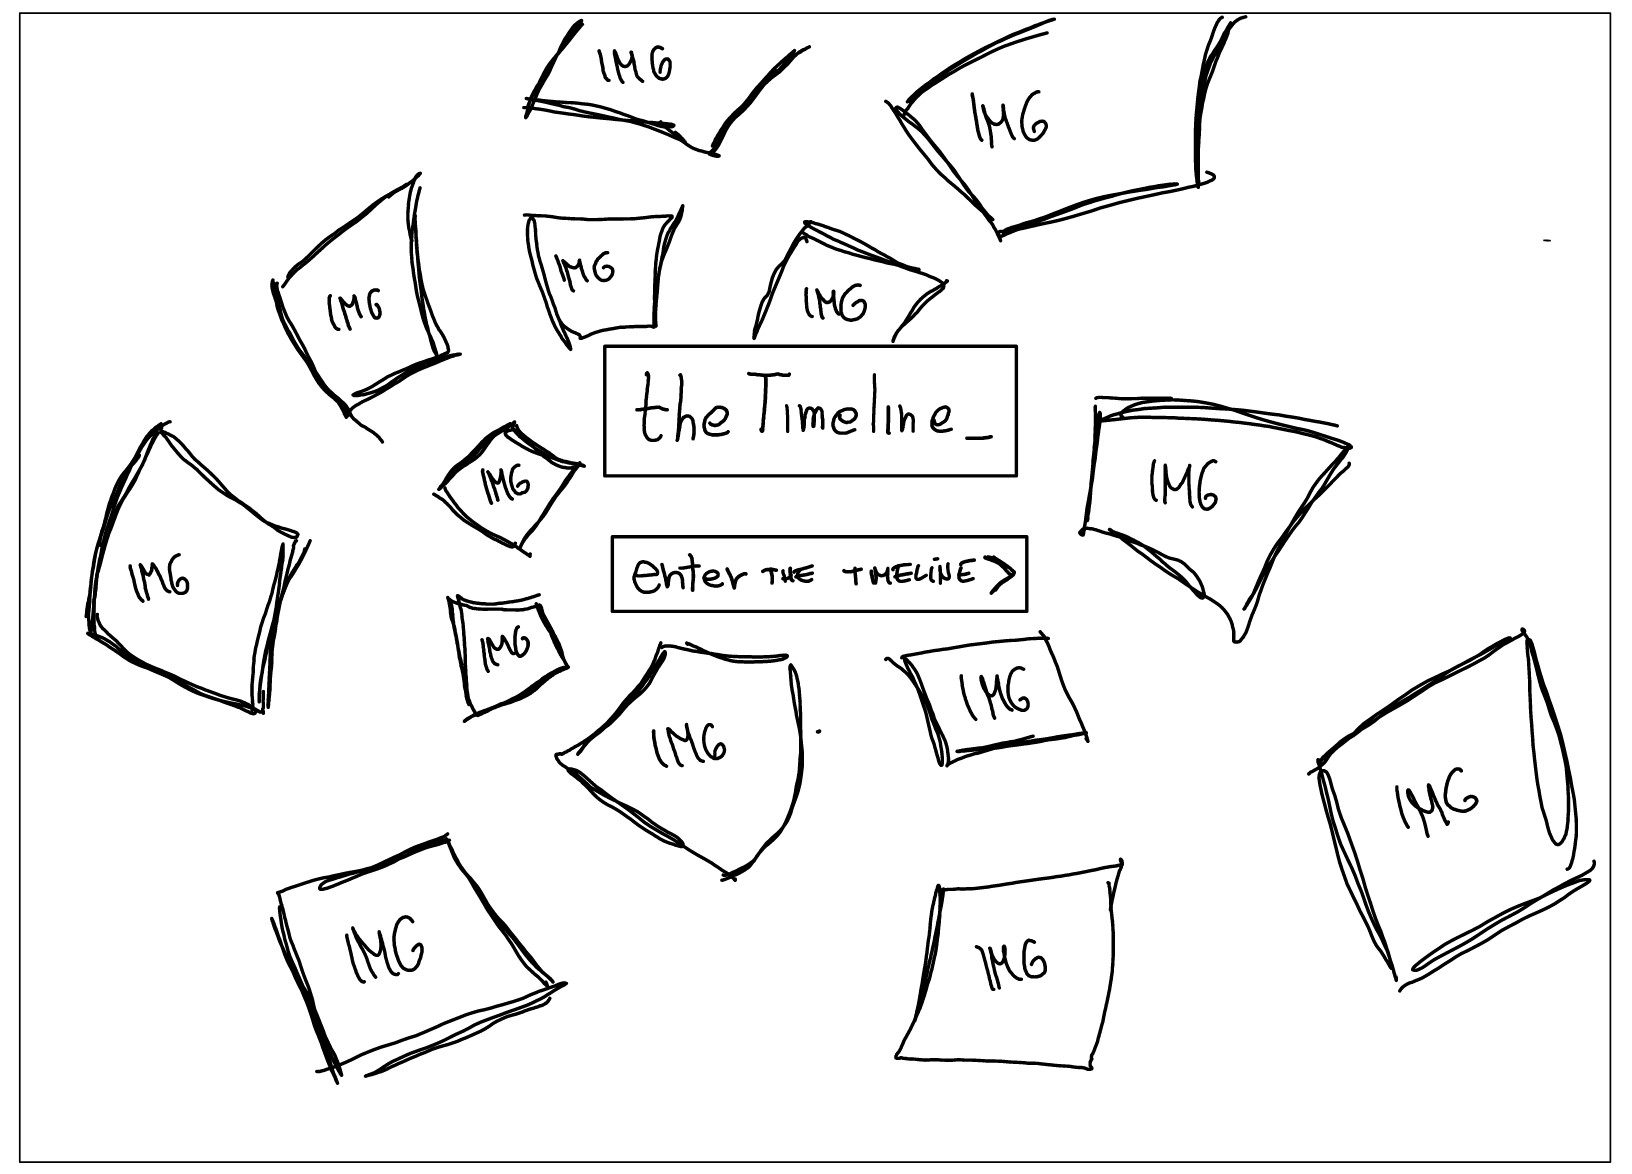
\includegraphics[width=.5\linewidth]{media/homepage_sketch.jpg}
        \end{figure}
        The homepage will feature many pictures taken from games arranged as a spiral, giving the idea of a journey through time.
        \newline
    \newpage
    \subsubsection{Timeline}
        \begin{figure}[h]
        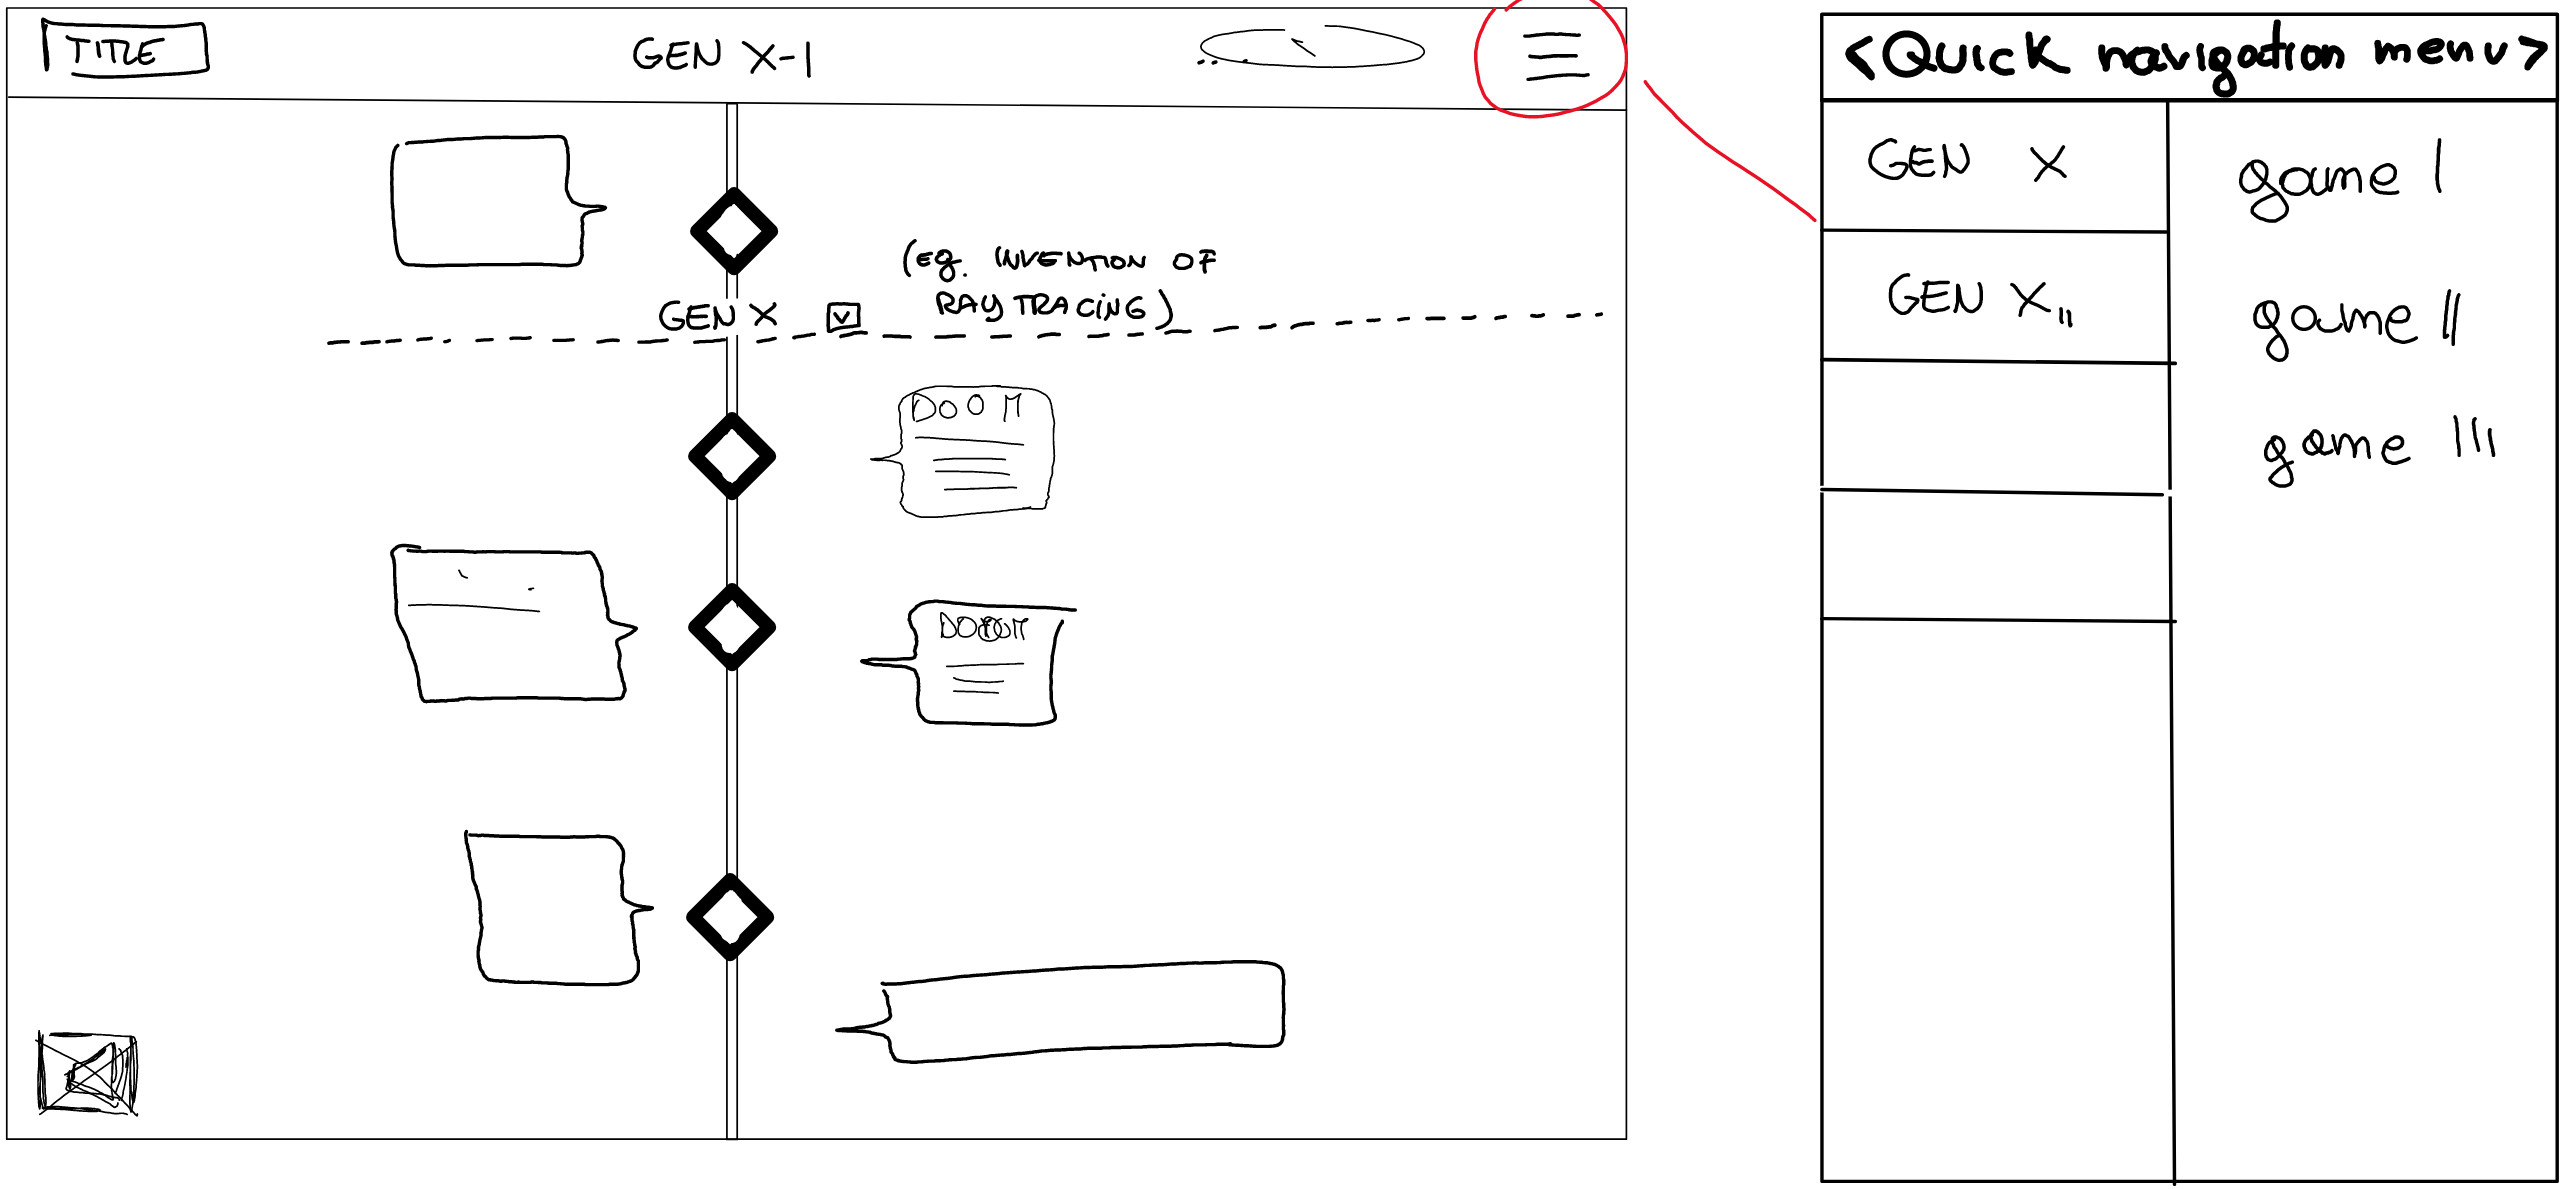
\includegraphics[width=.7\linewidth]{media/timeline_sketch.jpg}
        \end{figure}
        The idea is to make a vertical scrollable timeline that shows a brief summary for every page. Once a 'bubble' is clicked, the user is lead to the full page of the videogame/console.
    \subsubsection{Individual pages}
        \begin{figure}[h!]
        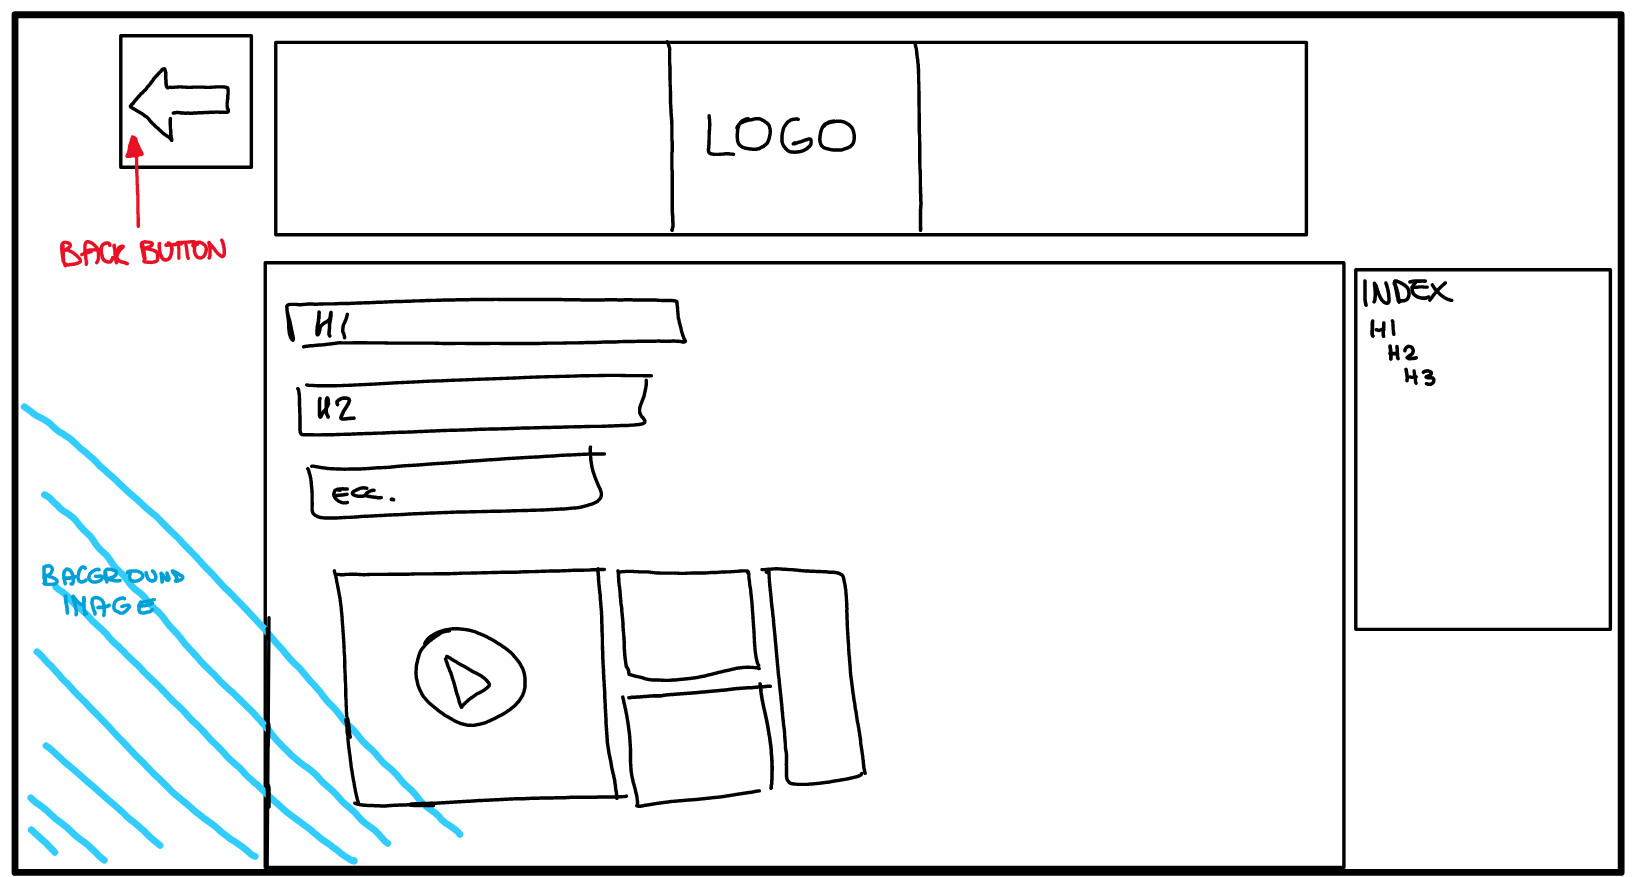
\includegraphics[width=.5\linewidth]{media/page_sketch.jpg}
        \end{figure}
        The videogame/console page shows the logo in the center and the actual content right under it. The page has the OST (Original Soundtrack) playing in background.
    \newpage
    \subsection{The CSS Masterplan}
        As the timeline progresses, the graphics of the page become more and more advanced (e.g at the beginning there are only black and white colors, then 24-bit colors ecc).
        For every generation of videogames that we cover there's going to be a stylesheet representing that generation's look and feel. The stylesheets will affect the timeline page but also the pages for videogames/console.\\\\
        Pages will use the CSS stylesheets that the CSS Leaders provide.
        \subsubsection{Example}
        
        \begin{figure}[h!]
            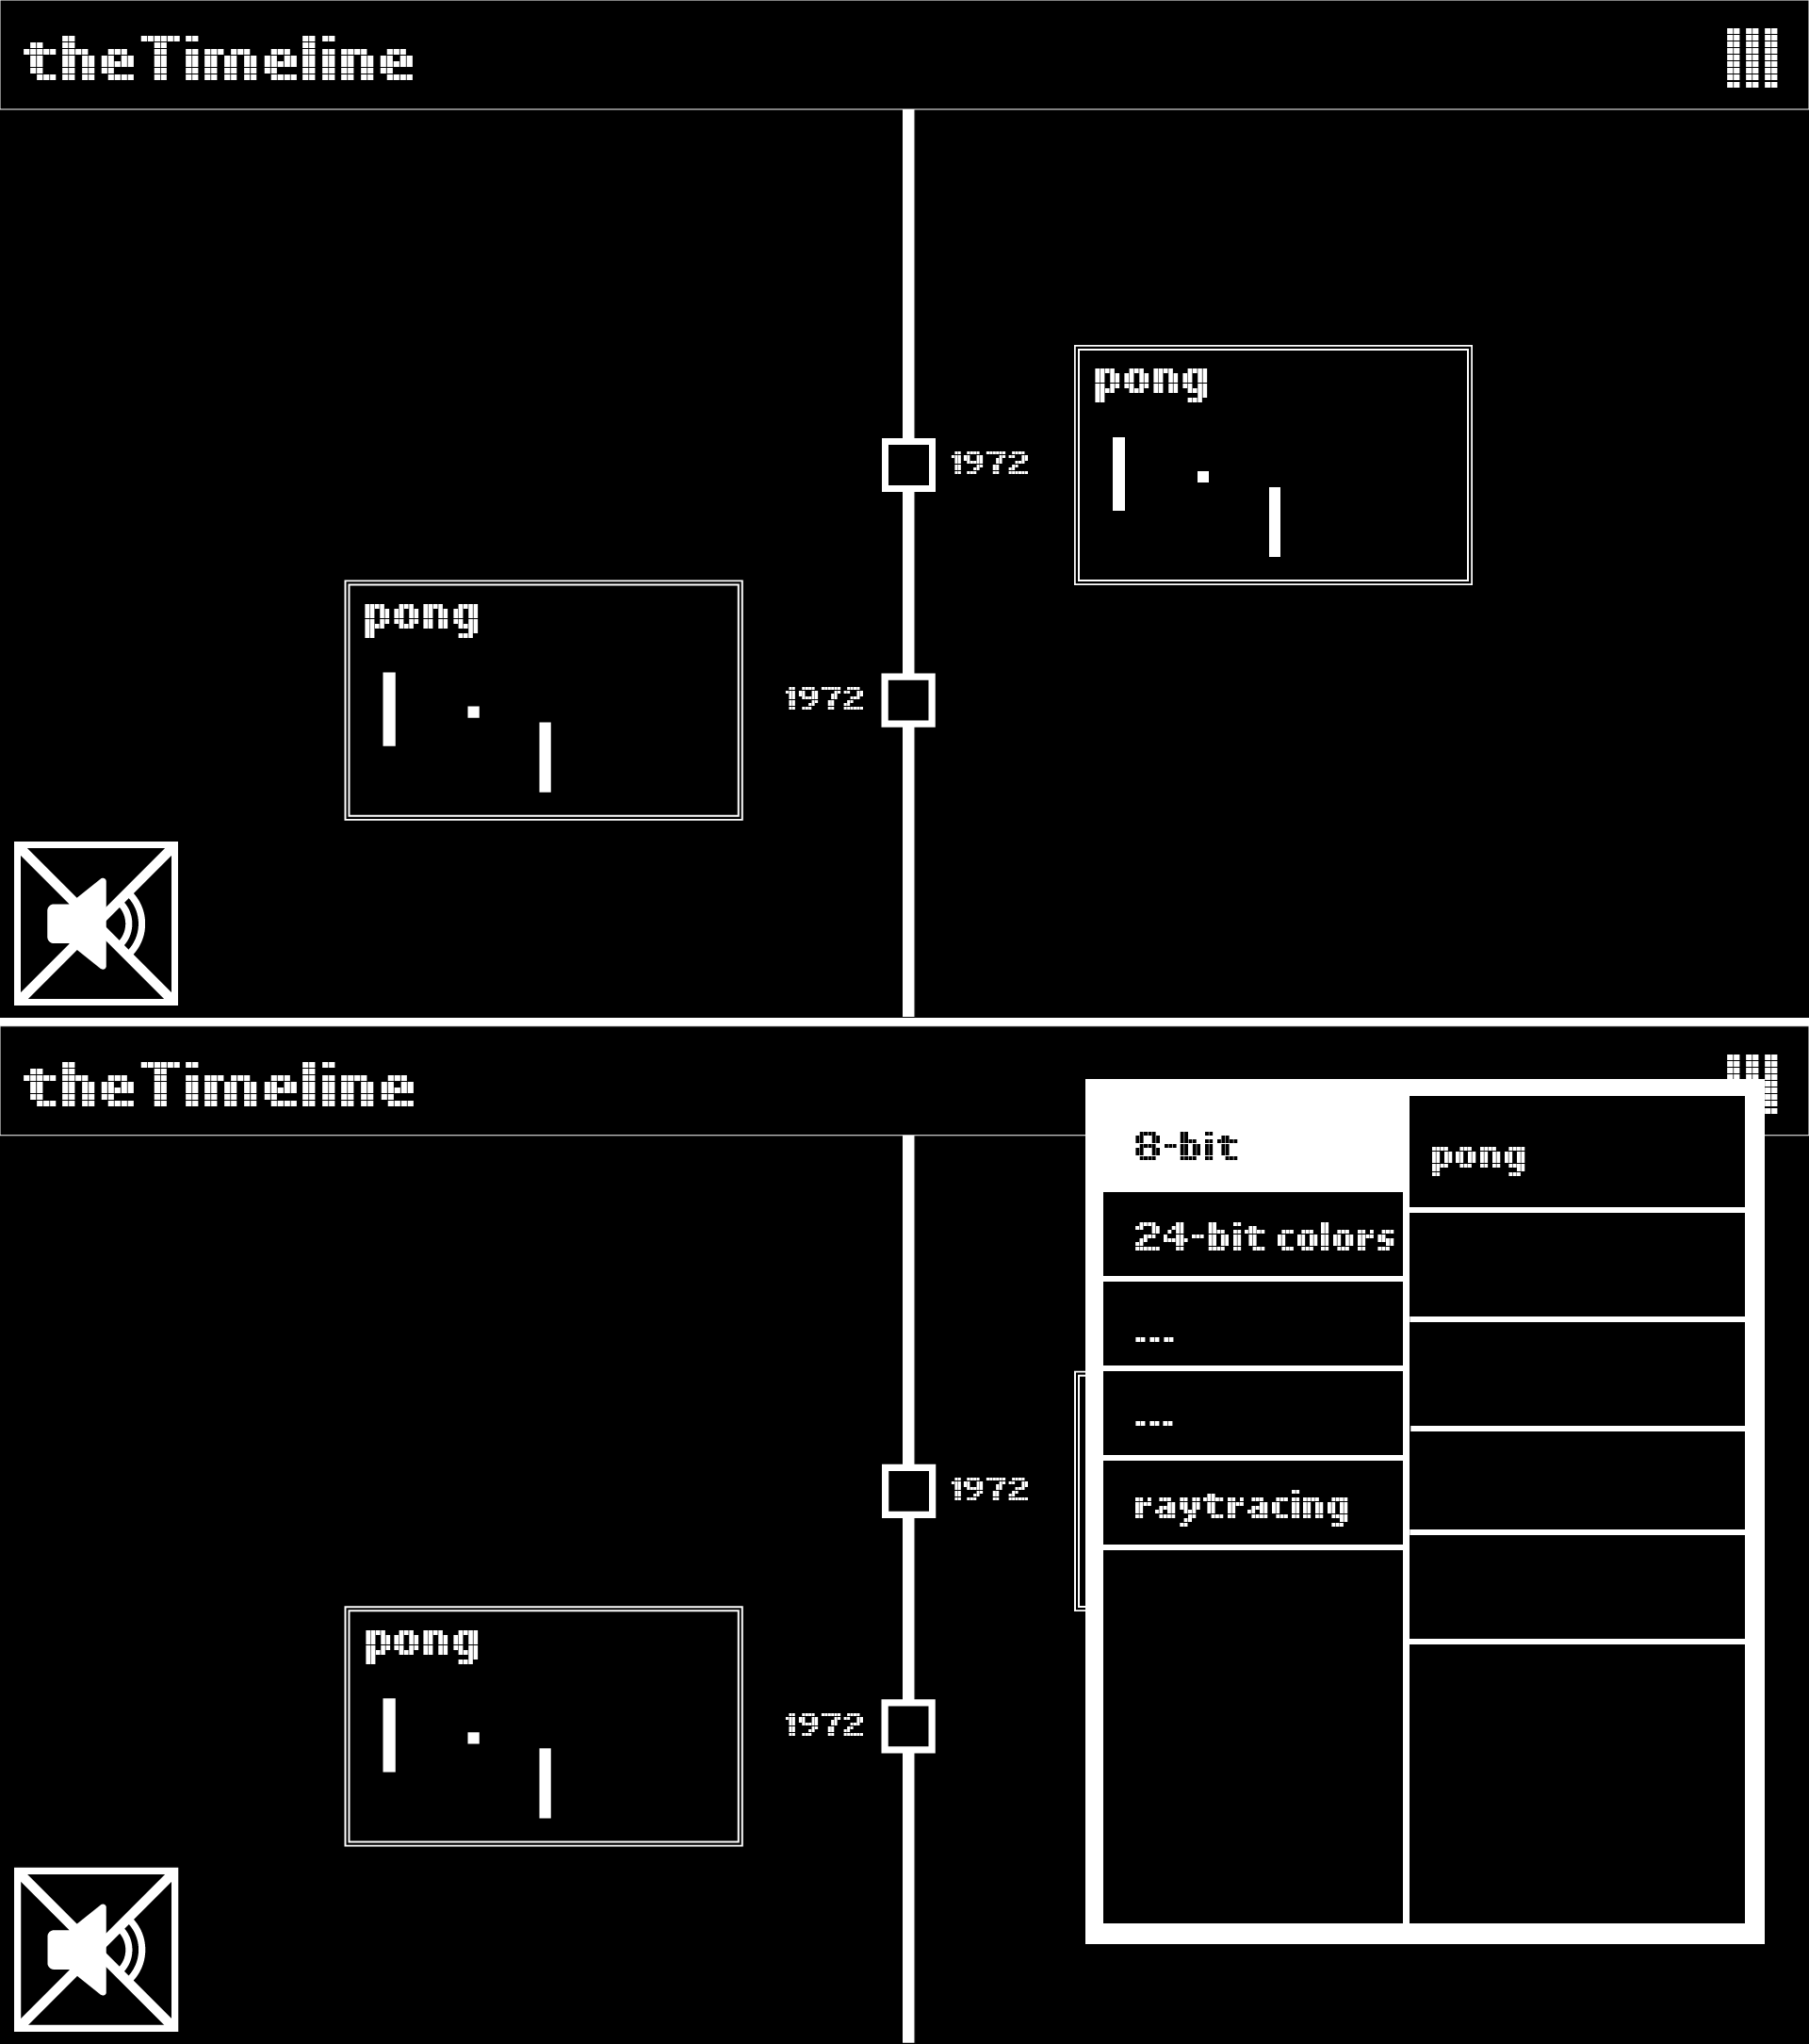
\includegraphics[width=.5\linewidth]{media/timeline_old.png}
            \caption{How the timeline looks during first generation}
        \end{figure}
    \subsection{Directory tree}
        \dirtree{%
        .1 pub.
        .2 documentation.
        .3 Official\underline{ }Documentation{.}pdf. 
        .2 web \ldots{..}\ldots{}\ldots{}\ldots{}\ldots{}\ldots{}\ldots{}\ldots{} \begin{minipage}[t]{0.8\linewidth}
                            The root of the webpage{.} Absolute paths start from here {.}
                            \end{minipage}. 
        .3 common\underline{ }media \ldots{}\ldots{}\ldots{}\ldots{}\ldots{} \begin{minipage}[t]{0.8\linewidth}
                            Media resources usable by everyone{.}
                            \end{minipage}.
        .4 audio.
        .4 gif.
        .4 images.
        .4 video.
        .3 styles \ldots{}\ldots{}\ldots{}\ldots{}\ldots{}\ldots{}\ldots{}\ldots{} \begin{minipage}[t]{0.8\linewidth}
                            All the stylesheets are located inside this directory{.}
                            \end{minipage}.
        .3 html \ldots{}\ldots{..}\ldots{}\ldots{}\ldots{}\ldots{}\ldots{} \begin{minipage}[t]{0.8\linewidth}
                            Every page has a folder inside this directory{.}
                            \end{minipage}. 
        .2 script.
        }
    \subsection{Example page}
        \dirtree{%
        .1  .
        .1 web \ldots{.....}\ldots{}\ldots{}\ldots{}\ldots{}\ldots{}\ldots{}\ldots{} \begin{minipage}[t]{0.8\linewidth}
                            The root of the webpage{.} Absolute paths start from here {.}
                            \end{minipage}.
        .2 html \ldots{..}\ldots{}\ldots{}\ldots{}\ldots{}\ldots{}\ldots{}\ldots{} \begin{minipage}[t]{0.8\linewidth}
                            Every page has a folder inside this directory{.}
                            \end{minipage}. 
        .3 \colorbox{yellow!30}{examplepage} \ldots{.}\ldots{}\ldots{}\ldots{}\ldots{} \begin{minipage}[t]{0.8\linewidth}
                            The directory of the page 'examplepage'{.}
                            \end{minipage}. 
        .4 \colorbox{yellow!30}{media} \ldots{..}\ldots{}\ldots{}\ldots{}\ldots{}\ldots{} \begin{minipage}[t]{0.8\linewidth}
                            Here goes all the media used by 'examplepage{.}html' {.}
                            \end{minipage}. 
        .4 \colorbox{yellow!30}{examplepage{.}html} \ldots{}\ldots{}\ldots{} \begin{minipage}[t]{0.8\linewidth}
                            The {.}html page{.}
                            \end{minipage}. 
        .3 {...} .
        }
        
        \subsubsection{Remarks}
            \begin{itemize}
            \item The folder and the .html file MUST have the same name!
            \item Please use the HTML template that we provide you in order to make sure the pages work with the stylesheets we also provide you.
            \item Manually change the CSS style only when really necessary and by keeping in mind the look of the generation the page is in.
            \end{itemize}
    \subsection{Good SVN practices}
        These are some guidelines to ensure the least possible amount of conflicts and clutter in the repository
        \begin{itemize}
            \item When you are about to start working, update the repository first to always make sure you have the latest version and there are no conflicts.
            \item \underline{To avoid conflicts, make sure you're the only one who is working on a certain file}. Conflicts take a lot of time to resolve.
            \item Always test your code and make sure it's working before making a commit. Always submit a working copy.
            \item Comment your code and commits.
        \end{itemize}
    
    
\end{document}
